

\section{Questão 4}

\subsubsection{Observe o conteúdo da tabela ARP. Diga o que significa cada uma das colunas.}

    \begin{figure}[H]
    \centering
    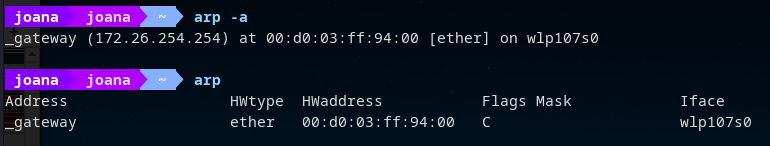
\includegraphics[width=350pt]{prints/Questao4/questao4-ArpTABLE.png}
    \caption{Tabela ARP.} \label{questao4-ARPRequest1}
    \end{figure}
    
    \par Uma tabela ARP é um método de armazenamento de informações descobertas através do protocolo ARP. É usada para registar os pares correspondentes de endereços MAC e endereços IP de dispositivos conectados a uma rede. Cada dispositivo conectado possui a sua própria tabela ARP, que, tal como referido acima, é responsável por armazenar os pares de endereços com os quais um determinado dispositivo já comunicou. Assim, apresentamos uma descrição das várias colunas presentes na tabela ARP.
    
    \begin{center}
        \begin{tabular}{|c|c|}
        \hline
            \cline{1-2}
            Coluna & Descrição  \\
            \hline \hline
            Address & endereço IP destino na rede\\
            HWtype & tipo de \textit{hardware} \\
            HWaddress & endereço MAC do \textit{hardware}\\
            Flags* & informação sobre a entrada \\
            Mask & máscara a aplicar ao endereço IP \\
            Iface & interface de saída \\
            \cline{1-2}
        \end{tabular}
    \end{center}
    
    \par \textbf{*} Neste caso, o valor da coluna é 'C'. Este tipo de entrada é visto quando as entradas são dinamicamente aprendidas pelo protocolo ARP.


    
    





\subsubsection{Qual é o valor hexadecimal dos endereços origem e destino na trama Ethernet que contém a mensagem com o pedido ARP (ARP Request)? Como interpreta e justifica o endereço destino usado?}

    \begin{figure}[H]
    \centering
    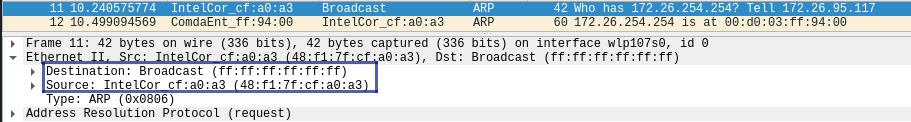
\includegraphics[width=500pt]{prints/Questao4/questao4-firstARP.png}
    \caption{Captura da Trama \textit{Ethernet} com pedido ARP.} \label{questao4-ARPRequest2}
    \end{figure}
    
    \begin{multicols}{2}
    \begin{itemize}
        \item MAC Origem: \textbf{48:f1:7f:cf:a0:a3}  
        \item MAC Destino: \textbf{ff:ff:ff:ff:ff:ff}
    \end{itemize}
    \end{multicols}


    \par A utilização do endereço MAC destino com o valor dos \textit{bits} todos a 1, é uma particularidade do protocolo ARP, isto é, como apagamos a \textit{cache} da tabela ARP, esta não tem qualquer informação de tradução e correspondência entre endereços IP e endereços MAC. Assim, quando, como neste caso, queremos enviar algum pacote para outro dispositivo, temos de primeiro descobrir o seu endereço MAC. Este problema é solucionado colocando o endereço MAC destino com todos os \textit{bits} a 1, representando uma mensagem em \textbf{\textit{broadcast}} (contendo o endereço IP do dispositivo alvo). 
    \par O modo de funcionamento pode ser caracterizado como uma difusão do pedido de \textit{broadcast} do nosso dispositivo por todos os nodos da mesma rede local até encontrar o aparelho que contém o mesmo endereço IP que o endereço IP destino do pedido. De seguida, o aparelho destino (alvo) envia uma resposta (ARP \textit{reply}) à nossa máquina contendo o seu endereço MAC.



\subsubsection{Qual o valor hexadecimal do campo tipo da trama Ethernet? O que indica?}

    \par O valor do campo \textit{type} do cabeçalho da trama \textit{Ethernet} é \textbf{0x0806} que indica que o protocolo encapsulado pela trama é o protocolo ARP.




\subsubsection{Como pode confirmar que se trata efetivamente de um pedido ARP? Identifique que tipo de endereços estão contidos na mensagem ARP? Que conclui?}

    \begin{figure}[H]
    \centering
    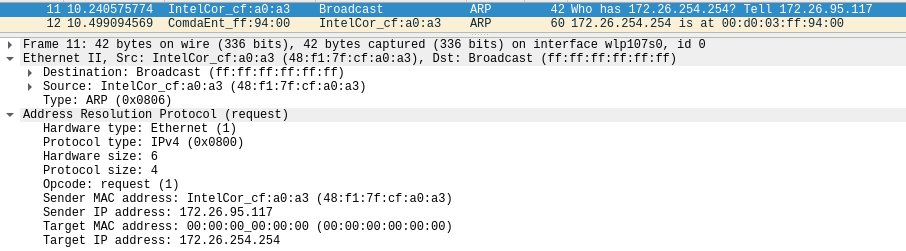
\includegraphics[width=500pt]{prints/Questao4/questao4-firstARP.png.png}
    \caption{Conteúdo ARP.} \label{questao4-ARPRequest-Extended}
    \end{figure}
    
    \paragraph{}
    \par Podemos confirmar que se trata de um pedido ARP pela análise do conteúdo da mensagem ARP, nomeadamente no valor do campo \textit{\textbf{Opcode}}. Este campo indica que tipo de mensagem ARP estamos a tratar, tendo, neste caso, o valor 1 que corresponde a um \textit{\textbf{request}}.
    
    \par Os endereços contidos na mensagem ARP são endereços MAC e IP dos sistemas de origem e destino, ou seja, para cada sistema está indicado o seu endereço IP e correspondente endereço MAC. No entanto, como podemos ver pela Figura \ref{questao4-ARPRequest-Extended}, esta possui o valor do endereço MAC destino (\textit{Target MAC Address}) a zeros. Isto acontece porque, como referido anteriormente, o endereço MAC destino é uma incógnita, sendo, exatamente, o que o protocolo  ARP está a tentar resolver.




\subsubsection{Explicite que tipo de pedido ou pergunta é feita pelo host de origem.}

    \par O \textit{host} de origem envia um pedido (ARP \textit{request}) a todos os nodos presentes na mesma LAN com o objetivo de obter uma resposta (ARP \textit{reply}) do sistema cujo endereço IP corresponde ao endereço IP destino presente na mensagem enviada, contendo esta, também, o endereço MAC do sistema alvo.


\subsubsection{Localize a mensagem ARP que é a resposta ao pedido ARP efetuado. (1) Qual o valor do campo ARP \textit{opcode}? O que especifica? (2) Em que campo da mensagem ARP está a resposta ao pedido ARP? }

    \begin{figure}[H]
    \centering
    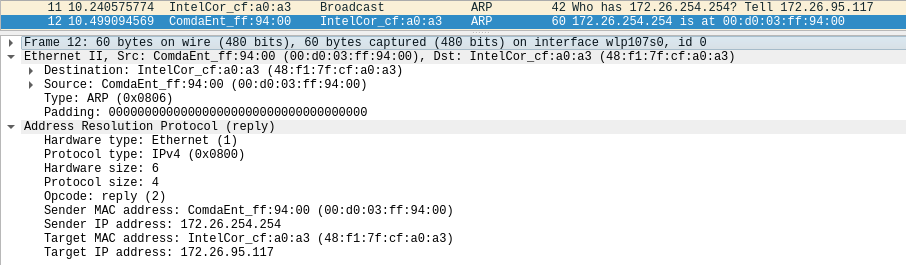
\includegraphics[width=500pt]{prints/Questao4/questao4-responseARP.png}
    \caption{Captura da Trama \textit{Ethernet} com resposta ARP.} \label{questao3-ARPResponse}
    \end{figure}
    
    \
    \par \textbf{(1)} O valor do campo \textit{Opcode} é 2 que corresponde a uma mensagem do tipo \textit{\textbf{ARP reply}}, ou seja, é uma mensagem de resposta a um pedido (\textit{request}) ARP.
    
    \par \textbf{(2)} O conteúdo da resposta ao pedido ARP está presente no campo \textbf{\textit{Sender MAC Address}}, onde podemos denotar a introdução de um endereço MAC válido, contrariamente ao presente no campo \textit{Target MAC Address} do ARP \textit{request} analisado anteriormente.




\newpage
\subsubsection{Na situação em que efetua um ping a outro host, assuma que este está diretamente ligado ao mesmo router, mas noutra subrede, e que todas as tabelas ARP se encontram inicialmente vazias. Esboce um diagrama em que indique claramente, e de forma cronológica, todas as mensagens ARP e ICMP trocadas, até à recepção da resposta ICMP do host destino.}


    \begin{figure}[H]
    \centering
    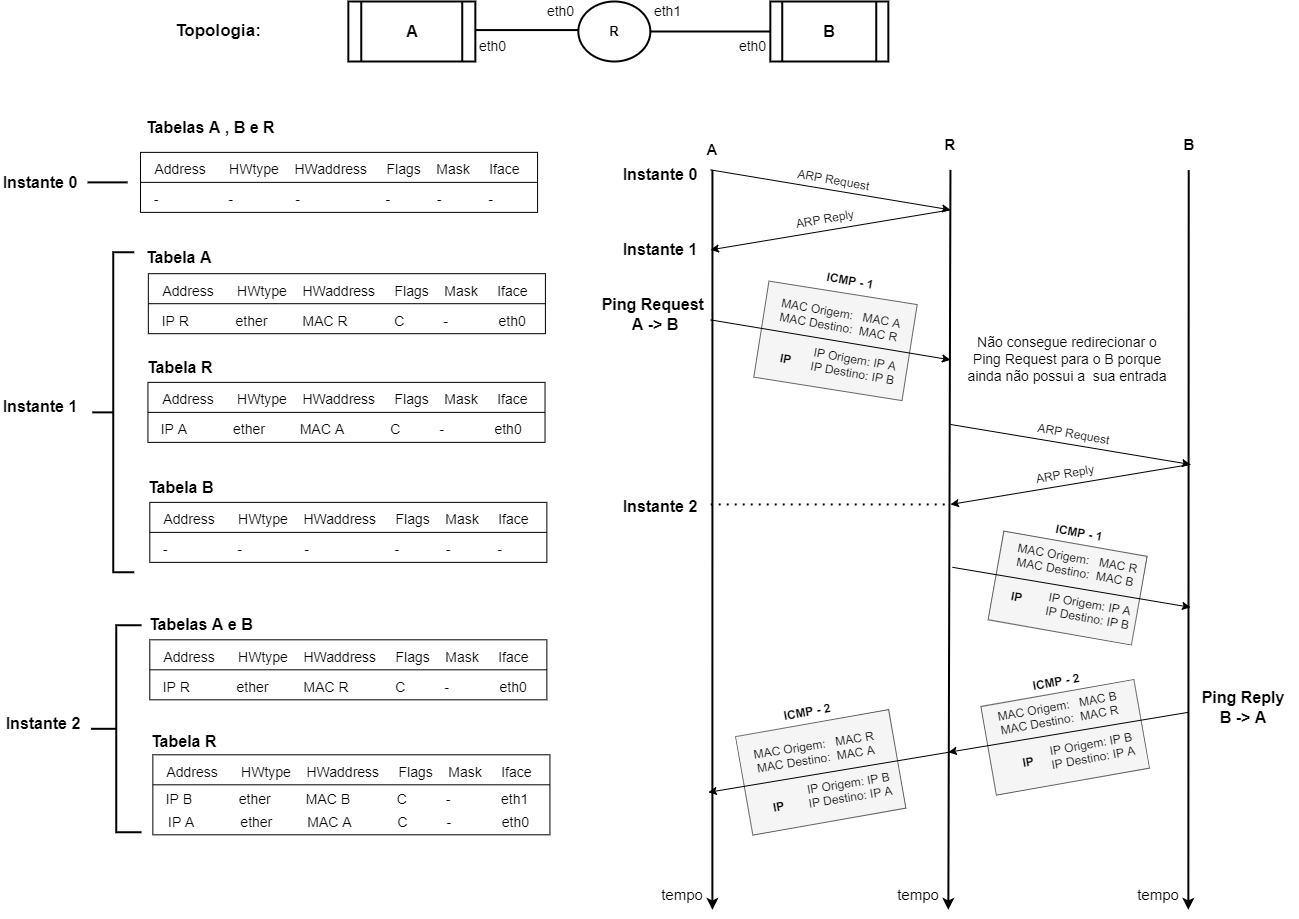
\includegraphics[width=\linewidth]{prints/Questao5/diagramaNOVO.png}
    \end{figure}